\majorheading{CHƯƠNG 3. THỬ NGHIỆM VÀ ĐÁNH GIÁ}

\section{3.1. Thiết lập thực nghiệm}

Mục đích của thí nghiệm ở Sprint 1 là kiểm chứng toàn bộ chuỗi truy xuất lai rồi sinh câu trả lời có trích dẫn có chạy được hay không, và đo sơ bộ hành vi của chuỗi này; đây không phải phép đo chất lượng của hệ thống hoàn chỉnh. Kế hoạch ban đầu dùng 200 trang mẫu do nhóm dữ liệu thu thập. Vì các trang này chưa được làm sạch và chưa có chỉ mục, thí nghiệm dùng tập dữ liệu khác: 240 bản ghi đầu tiên của tệp \texttt{armors.csv}, tệp có 568 bản ghi tại thời điểm đọc (25/10/2026). Mỗi bản ghi mô tả một món trang phục với tên, loại, khối lượng và đoạn mô tả lấy từ trò chơi. Đây là một phép thử trên tập con, không thay thế việc chạy trên dữ liệu đã xử lý của nhóm dữ liệu. Bảng \ref{tab:cauhinh} nêu cấu hình.


\tabbegin{Cấu hình thí nghiệm cơ sở}{tab:cauhinh}
\begin{longtable*}{|C{0.30}|C{0.70}|}
\hline \textbf{Hạng mục} & \textbf{Giá trị} \\ \hline
Dữ liệu & 240 bản ghi đầu của \texttt{armors.csv} theo thứ tự tệp, không xáo trộn, không bỏ bản ghi \\ \hline
Đơn vị lập chỉ mục & Mỗi bản ghi là một tài liệu và một điểm trong Qdrant; nội dung truy xuất gồm tên, loại, khối lượng và mô tả \\ \hline
Embedding & \texttt{multilingual-e5-small} qua FastEmbed (ONNX), 384 chiều; tiền tố \texttt{passage:} và \texttt{query:} thêm đúng một lần; đầu vào dài nhất 123 token, không phải rút gọn \\ \hline
Từ khóa & BM25 tiếng Anh dạng vector thưa, bật hiệu chỉnh IDF \\ \hline
Hợp nhất & Truy vấn nhiều giai đoạn của Qdrant với RRF, tham số mặc định; lấy 5 kết quả đầu \\ \hline
Kho vector & Qdrant ở chế độ bộ nhớ, tạo mới cho mỗi lần chạy \\ \hline
Mô hình sinh & \texttt{deepseek-flash}, tắt chế độ suy luận, tối đa 512 token đầu ra \\ \hline
Chưa có trong thí nghiệm & Viết lại và dịch truy vấn, xếp hạng lại, lọc theo phạm vi, tìm web \\ \hline
Câu hỏi & 10 câu về trang phục: 5 tiếng Việt và 5 tiếng Anh, chọn từ các bản ghi đã biết có trong tập \\ \hline
Đáp án tham chiếu & Lấy từ chính nội dung CSV, không đưa vào chỉ mục hay lời nhắc \\ \hline
Thư viện & fastembed 0.9.0, qdrant-client 1.19.1, openai 3.33.0, onnxruntime 1.31.0, tokenizers 0.23.3 \\ \hline
\end{longtable*}
\tabend


Lời nhắc yêu cầu trả lời thẳng, thường từ một đến ba câu, đúng ngôn ngữ câu hỏi, giữ tên riêng gốc, dẫn nguồn theo số trong năm kết quả đầu, và giữ sắc thái như ``được đồn là'' của nguồn. Nguồn trích dẫn được ghi là tệp dữ liệu kèm số thứ tự bản ghi, không tự tạo địa chỉ trang wiki. Lượt chạy được chấm có mã \texttt{20261025T144625694379Z} và chạy ngày 25/10/2026. Thời gian lập vector cho 240 bản ghi là 4,6 giây trên máy phát triển.


Việc chấm điểm được thực hiện thủ công theo thang 0, 1, 2 cho độ đúng (trả lời đúng và đủ ý được hỏi) và độ bám nguồn (mọi khẳng định được hỗ trợ bởi đoạn đã truy xuất). Người chấm là một trợ lý trí tuệ nhân tạo hỗ trợ nhóm, đối chiếu câu hỏi, đáp án tham chiếu và các đoạn đã lưu mà không chạy lại mô hình. Đây không phải chấm điểm độc lập của người thứ hai hay của một mô hình khác, và việc đối chiếu chỉ dựa trên nội dung tệp dữ liệu chứ chưa so với trò chơi.


\section{3.2. Kết quả truy xuất}

Bảng \ref{tab:truyxuat} tổng hợp kết quả truy xuất. Một tài liệu được xem là đúng khi nó là bản ghi chứa câu trả lời của câu hỏi. Chỉ số trích dẫn hợp lệ nghĩa là các số hiệu trong câu trả lời trỏ đến đoạn có thật trong năm đoạn được đưa vào lời nhắc; chỉ số này chưa chứng minh câu trả lời được nguồn hỗ trợ.


\tabbegin{Kết quả truy xuất và sinh trả lời của thí nghiệm cơ sở}{tab:truyxuat}
\begin{longtable*}{|C{0.18}|C{0.10}|C{0.12}|C{0.12}|C{0.16}|C{0.16}|C{0.16}|}
\hline \textbf{Ngôn ngữ} & \textbf{Số câu} & \textbf{Hit@5} & \textbf{MRR@5} & \textbf{Trích dẫn hợp lệ} & \textbf{Truy xuất (ms)} & \textbf{Sinh (ms)} \\ \hline
Tiếng Việt & 5 & 5/5 & 0,700 & 5/5 & 19,9 & 1.100,8 \\ \hline
Tiếng Anh & 5 & 5/5 & 0,900 & 5/5 & 17,4 & 995,2 \\ \hline
\textbf{Chung} & \textbf{10} & \textbf{10/10} & \textbf{0,800} & \textbf{10/10} & --- & --- \\ \hline
\end{longtable*}
\tabend


Độ trễ là trung bình do notebook ghi lại trong một lượt chạy duy nhất trên máy phát triển, với Qdrant trong bộ nhớ và một tập chỉ 240 điểm. Con số này chỉ cho biết bậc độ lớn; nó không đại diện cho độ trễ khi chạy trên máy chủ thật với kho dữ liệu lớn hơn, bước viết lại và bước xếp hạng lại.


\begin{figure}[H]\centering
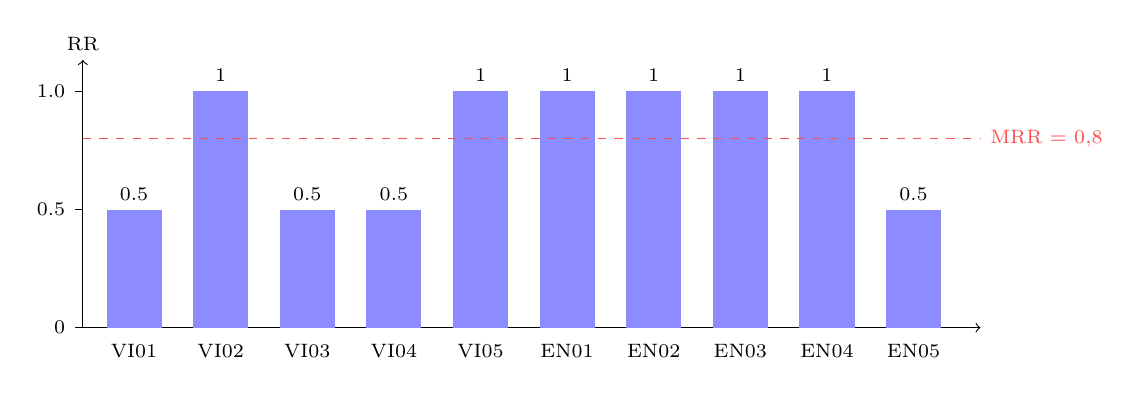
\begin{tikzpicture}
  \draw[->] (0,0) -- (0,3.4) node[above,font=\scriptsize] {RR};
  \draw[->] (0,0) -- (11.4,0);
  \foreach \y in {0,0.5,1.0} {\draw (0,\y*3) -- (-0.1,\y*3) node[left,font=\scriptsize] {\y};}
  \foreach \n/\v [count=\i from 0] in {VI01/0.5, VI02/1, VI03/0.5, VI04/0.5, VI05/1, EN01/1, EN02/1, EN03/1, EN04/1, EN05/0.5} {
    \pgfmathsetmacro{\x}{0.3+\i*1.1}
    \fill[blue!45] (\x,0) rectangle ++(0.7,\v*3);
    \node[font=\scriptsize] at (\x+0.35,-0.3) {\n};
    \node[font=\scriptsize] at (\x+0.35,\v*3+0.2) {\v};
  }
  \draw[dashed,red!70] (0,2.4) -- (11.4,2.4) node[right,font=\scriptsize,red!70] {MRR = 0,8};
\end{tikzpicture}
\caption{Nghịch đảo thứ hạng (RR) của tài liệu đúng đầu tiên cho từng câu hỏi}\label{fig:rr}
\end{figure}


Cả 10 câu đều có tài liệu đúng trong năm kết quả đầu. Với bốn câu (VI01, VI03, VI04 và EN05) tài liệu đúng nằm ở hạng hai, còn hạng một là một biến thể hoặc một món khác trong cùng bộ. Ví dụ, với câu hỏi về chủ nhân của All-knowing Armor, hạng một là bản ``altered'' chỉ có mô tả ``phiên bản nhẹ hơn'', còn bản gốc chứa tên Gideon Ofnir nằm ở hạng hai. Các bản ghi cùng tên bộ giáp có vector và từ khóa giống nhau nên dễ chiếm các vị trí đầu. Mô hình sinh vẫn chọn được nguồn đúng trong số năm đoạn và trích dẫn nó, nhưng nếu giảm số đoạn đưa vào lời nhắc, những câu này sẽ gặp rủi ro. Đây là chỗ bước xếp hạng lại có thể cải thiện.


Cần đọc kết quả này một cách thận trọng. Các câu hỏi tiếng Việt đều chứa nguyên tên tiếng Anh của món trang phục, và trong thí nghiệm này câu hỏi không được dịch trước khi đưa vào BM25, nên phần từ khóa có thể khớp nhờ tên riêng. Vì vậy kết quả không cho phép kết luận về khả năng truy xuất chéo ngôn ngữ đối với câu hỏi tiếng Việt không chứa tên tiếng Anh. Thí nghiệm cũng chưa chạy riêng từng thành phần (chỉ vector, chỉ từ khóa) nên chưa đo được đóng góp của việc kết hợp.


\section{3.3. Đánh giá câu trả lời}

Bảng \ref{tab:tungcau} nêu điểm và nhận xét cho từng câu. Điểm cho mỗi tiêu chí tối đa là 2; tổng độ đúng là 20 trên 20 và tổng độ bám nguồn là 20 trên 20.


\tabbegin{Điểm và nhận xét theo từng câu hỏi (thang 0--2)}{tab:tungcau}
\begin{longtable*}{|C{0.08}|C{0.09}|C{0.09}|C{0.09}|C{0.65}|}
\hline \textbf{Câu} & \textbf{Hạng nguồn đúng} & \textbf{Đúng} & \textbf{Bám nguồn} & \textbf{Nhận xét} \\ \hline
VI01 & 2 & 2 & 2 & Đúng người mặc là Gideon Ofnir; trích đúng bản gốc, không nhầm sang bản altered ở hạng một \\ \hline
VI02 & 1 & 2 & 2 & Đúng ``đọc vận mệnh trong các vì sao''; thêm một câu về hậu duệ của glintstone sorcerers có trong nguồn nhưng không được hỏi \\ \hline
VI03 & 2 & 2 & 2 & Đúng hiệu ứng che tiếng bước chân; cách dịch ``làm nghẹt'' chưa tự nhiên, nên dùng ``làm giảm'' \\ \hline
VI04 & 2 & 2 & 2 & Đúng gia đình hoàng gia Carian; trích đúng Carian Knight Armor thay vì Gauntlets ở hạng một \\ \hline
VI05 & 1 & 2 & 2 & Đúng nhóm quý tộc ở kinh đô; câu thứ hai về Shattering có trong nguồn nhưng thừa; cách dịch ``undead'' cần chính xác hơn \\ \hline
EN01 & 1 & 2 & 2 & Đủ hai ý được hỏi: người mặc và việc run sợ khi nhìn vào ý chí của Queen Marika \\ \hline
EN02 & 1 & 2 & 2 & Đúng khác biệt: bản altered nhẹ hơn (3,2 so với 4,1); trích đúng hai biến thể \\ \hline
EN03 & 1 & 2 & 2 & Nêu đúng ý ``the night sky no longer cradles fate''; thêm phần hậu duệ glintstone sorcerers không cần thiết \\ \hline
EN04 & 1 & 2 & 2 & Giữ đúng sắc thái ``được đồn là Numen'', không biến tin đồn thành sự thật \\ \hline
EN05 & 2 & 2 & 2 & Xác định đúng man-wolf Blaidd; thêm câu về Gauntlets không cần thiết \\ \hline
\end{longtable*}
\tabend


Kết quả cho thấy mô hình bám khá sát nguồn: không có khẳng định nào ngoài nội dung được truy xuất, các sắc thái như ``được đồn là'' được giữ, và khi không có đủ thông tin cho phần nào đó (câu EN02) mô hình ghi rõ các bản ghi không nêu thêm khác biệt. Mô hình cũng xử lý được cặp đa ngôn ngữ: câu hỏi tiếng Việt về nguồn tiếng Anh được trả lời bằng tiếng Việt với tên riêng giữ nguyên.


Điểm tuyệt đối 20/20 không nên được hiểu là chất lượng 100\% của chatbot. Các câu hỏi được chọn từ những món đã biết có trong tập, không có câu không thể trả lời, không có câu cần ghép nhiều nguồn, và mỗi đáp án tham chiếu nằm gọn trong một đoạn mô tả ngắn. Người chấm không độc lập và nguồn chưa được kiểm chứng với trò chơi. Với mẫu 10 câu, một câu sai làm điểm giảm 10 điểm phần trăm, nên không thể ước lượng đáng tin cậy tỉ lệ đúng của hệ thống.


\section{3.4. Phân tích lỗi và khả năng khái quát hóa}

Thí nghiệm không có câu trả lời sai, nhưng các quan sát ghi nhận được là:


\begin{itemize}
\item \textbf{Thông tin thừa (4 câu: VI02, VI05, EN03, EN05).} Mô hình thêm chi tiết đúng nguồn nhưng không được hỏi. Hướng xử lý là bổ sung vào lời nhắc yêu cầu chỉ trả lời khía cạnh được hỏi, rồi đánh giá lại để xem tác động.
\item \textbf{Dịch chưa tự nhiên (VI03, VI05).} Cần kiểm tra ở quy mô lớn hơn vì chỉ vài câu bị ảnh hưởng.
\item \textbf{Biến thể chiếm hạng đầu (4 câu).} Cần so sánh thêm xếp hạng lại và cách ghép tên chính xác.
\item \textbf{Chưa có phép thử các tình huống khó:} câu không có đáp án, câu không chứa nguyên tên tài liệu, câu diễn đạt lại, câu dễ nhầm biến thể, câu cần ghép nhiều nguồn.
\end{itemize}


Về khả năng khái quát, kết quả hiện chỉ hợp lệ cho đúng tập 240 bản ghi này. Nội dung chính của dự án là văn xuôi dài trong các trang wiki, được chia đoạn theo tiêu đề; số lượng đoạn lớn hơn nhiều, độ dài đoạn khác, và nhiều đoạn có nội dung gần nhau. Các điều kiện đó chưa được thử, nên cần chạy lại trên dữ liệu đã làm sạch cùng bộ câu hỏi chuẩn 30 câu trước khi nêu kết luận về chất lượng.


\section{3.5. Kiểm thử kỹ thuật và chất lượng phần mềm}

Ngoài thí nghiệm về mô hình, nhóm kiểm tra chất lượng của phần mềm nền tảng. Bảng \ref{tab:kiemthu} tổng hợp các kiểm tra chạy lại trên nhánh phát triển ngày 26/10/2026.


\tabbegin{Kết quả kiểm tra phần mềm trên nhánh phát triển}{tab:kiemthu}
\begin{longtable*}{|C{0.27}|C{0.43}|C{0.30}|}
\hline \textbf{Thành phần} & \textbf{Kiểm tra} & \textbf{Kết quả} \\ \hline
Phụ trợ (backend) & Công cụ kiểm tra và định dạng mã (117 tệp) & Đạt \\ \hline
Phụ trợ (backend) & Kiểm thử đơn vị: cấu hình, nhật ký, middleware, kiểm tra sức khỏe, vòng đời tài nguyên, quy ước cổng & 79 đạt \\ \hline
Phụ trợ (backend) & Kiểm thử tích hợp với PostgreSQL, Redis, Qdrant thật & Đạt trong tích hợp liên tục \\ \hline
Website & Định dạng, biên dịch; 8 kiểm thử về luồng SSE, mã hóa UTF-8, ngắt luồng, lỗi 429, nguồn lỗi, ngôn ngữ (Node 24.22.0) & Đạt; 8 đạt trên 8 \\ \hline
Bot Discord & Kiểm tra kiểu và định dạng & Đạt \\ \hline
Tích hợp liên tục & Bốn lần chạy gần nhất trên nhánh phát triển & Thành công \\ \hline
\end{longtable*}
\tabend


Quá trình này cũng giúp phát hiện và sửa một số lỗi thiết kế: tích hợp liên tục từng báo lỗi ở mọi yêu cầu hợp nhất do dòng mô tả mã quá dài; tệp cấu hình môi trường có chú thích cuối dòng bị công cụ dựng container hiểu thành giá trị; middleware ghi mã định danh yêu cầu bị mất khi truyền theo luồng nên đã viết lại ở mức ASGI; nhóm thống nhất không chạy tiến trình nào trên cổng mặc định của công cụ nên đặt quy ước cổng riêng, có kiểm thử chặn tái phạm. Các kiểm thử trên xác nhận phần nền tảng hoạt động đúng thiết kế; chúng không đo chất lượng hỏi đáp.


\section{3.6. Chương trình minh họa}

Nhóm cung cấp hai ứng dụng khách và một điểm thử phần phụ trợ. Trạng thái của từng phần được nêu ở Bảng \ref{tab:demo} để tránh nhầm giữa giao diện hoàn thiện và chức năng đã nối với dữ liệu thật.


\tabbegin{Các thành phần minh họa và trạng thái}{tab:demo}
\begin{longtable*}{|C{0.22}|C{0.78}|}
\hline \textbf{Thành phần} & \textbf{Trạng thái tại thời điểm báo cáo} \\ \hline
Website & Trang hỏi đáp với ô nhập, hiển thị Markdown, danh sách nguồn và hộp trích dẫn, lịch sử hội thoại của khách (lưu trong trình duyệt, tối đa 30 cuộc), nút phản hồi, trang giới thiệu nguồn và giấy phép, trang quản trị, chuyển ngôn ngữ Việt hoặc Anh, giao diện tối, thích ứng từ 360 px. Chế độ mặc định là xem thử với dữ liệu cố định có nhãn minh họa, không gọi mô hình. Chế độ kết nối API đọc luồng SSE thật nhưng phần phụ trợ chưa có điểm hỏi đáp \\ \hline
Bot Discord & Khung ứng dụng, đăng ký lệnh gạch chéo và lệnh kiểm tra \texttt{/ping}; các lệnh hỏi đáp mới là tệp khung \\ \hline
API phụ trợ & Điểm kiểm tra sức khỏe và điểm thử mô hình sinh (chỉ ở môi trường phát triển); tài liệu Swagger ở môi trường phát triển \\ \hline
Thí nghiệm RAG & Notebook cho phép chạy lại thí nghiệm cơ sở, kể cả bước gọi mô hình sinh nếu được bật \\ \hline
\end{longtable*}
\tabend


Để chạy các thành phần trên máy phát triển, cần khởi động hạ tầng bằng \texttt{docker compose up -d --wait postgres qdrant redis}, chạy API bằng lệnh \texttt{make api} (địa chỉ \texttt{http://127.0.0.1:18000/api/docs}) và chạy giao diện bằng \texttt{npm run dev} trong thư mục \texttt{web} (địa chỉ \texttt{http://localhost:15173}). Hướng dẫn đầy đủ nằm trong tệp README của kho mã [14].


\section{3.7. Kết luận và hướng phát triển}

Báo cáo trình bày thiết kế và kết quả giai đoạn đầu của Index Beast, hệ thống hỏi đáp lore Elden Ring dựa trên truy xuất lai và mô hình ngôn ngữ lớn. Kết quả đạt được gồm: một nền tảng phát triển có môi trường dựng lại được, kiểm tra tự động và cấu hình an toàn; quy trình thu thập dữ liệu ngoại tuyến đã tải thử 200 trang cùng 1.188 ảnh với kiểm tra toàn vẹn; chiến lược chia đoạn được đề xuất kèm số đo; bộ 30 câu hỏi chuẩn cho đánh giá; và một thí nghiệm cơ sở cho thấy chuỗi truy xuất lai rồi sinh có trích dẫn chạy được trên tập con dữ liệu, với Hit@5 là 10/10, MRR@5 là 0,8 và điểm 20/20 cho cả độ đúng lẫn độ bám nguồn trên 10 câu.


Những kết quả này có giới hạn rõ. Dữ liệu của thí nghiệm là 240 bản ghi dạng bảng chứ chưa phải văn xuôi đã làm sạch; chưa có bước viết lại truy vấn, xếp hạng lại hay tìm web; câu hỏi được chọn từ những mục đã biết và do một người chấm không độc lập; bộ câu hỏi chuẩn chưa được kiểm tra chéo; chưa so sánh các biến thể của quy trình; và các mục tiêu về độ trễ, chi phí, Recall@5 và độ đúng trên bộ chuẩn đều chưa được đo. Phạm vi nội dung theo từng mục (bản gốc hay bản mở rộng) và giấy phép của ảnh cũng chưa được rà soát xong.


Hướng phát triển theo kế hoạch gồm các bước sau. Sprint 2 hoàn thiện làm sạch, chia đoạn và lập chỉ mục trên toàn bộ dữ liệu, đồng thời chốt hợp đồng dữ liệu và hợp đồng giao diện lập trình. Sprint 3 nối quy trình từ đầu đến cuối với viết lại truy vấn, xếp hạng lại, sinh trả lời có trích dẫn, truyền theo luồng, và đo Recall cùng MRR trên bộ chuẩn. Sprint 4 bổ sung bộ chấm tự động có đối chiếu với người chấm, tối ưu tham số truy xuất, chặn tấn công qua lời nhắc, giới hạn tần suất và tìm web dự phòng. Sprint 5 triển khai thật và kiểm thử tải theo các mục tiêu độ trễ. Sprint 6 kiểm thử với người dùng thật, sửa lỗi và bàn giao. Ở mỗi giai đoạn, kết quả cần được ghi cùng điều kiện đo, phiên bản dữ liệu và mã nguồn để người khác kiểm tra lại được.
